%\addcontentsline{toc}{section}{Unnumbered Section}
\chapter{Tools} \label{chap:tools}

In this project all tools and elaborations were made in GNU/Linux environment.
We had two available remote computers, to which we connect by \texttt{ssh} command on terminal.\\
In particular we worked on the following machines:
	\begin{enumerate}
		\item \textbf{Local host}
		\begin{itemize} 
			\item Ubuntu 14.04 LTS, (4.4.0-148-generic x86\_64)
			\item 1 CPU Intel® Core™ i5 CPU M 450 @ 2.40GHz x 4 
		\end{itemize}
		
		\item \textbf{P100 remote server}
		\begin{itemize}
			\item Ubuntu 18.04.2 LTS (4.15.0-43-generic x86\_64)	
			\item 80 CPUs Intel(R) Xeon(R) CPU E5-2698 v4 @ 2.20GHz		
			\item 4 GPUs Tesla P100-PCIE-16GB\\\\
		\end{itemize}
		 
		\item\textbf{ M40 remote server}
		\begin{itemize}
			\item Ubuntu 16.04.6 LTS (4.4.0-154-generic x86\_64)
			\item 48 CPUs Intel(R) Xeon(R) CPU E5-2670 v3 @ 2.30GHz
			\item 4 GPUs NVIDIA Tesla M40\\
		\end{itemize}
	\end{enumerate}
	Given that this work is focused on the use of the remote GPUs, their main specifics are listed in Table \ref{tab:gpuspecs}. All the following informations have been get by executing \texttt{cudaDeviceQuery} application (located inside samples of CUDA Toolkit).\\
	\begin{table}	
	\begin{tabular}{|c | c c |} 
		\hline
  & \textbf{Tesla P100} & \textbf{Tesla M40} \\ [0.5ex] 
		\hline\hline
		
		\textbf{Driver/Runtime Version} & 10.1  & 10.1 \\ 
		\hline
		
		\textbf{CUDA Capability} & 6.0 & 5.2 \\
		\hline
		\textbf{\makecell{Tot. \\global memory amount}} & 16281 MBytes & 11449 MBytes \\
		\hline
		
		\textbf{Multiprocessors} & 56 & 24 \\
		\hline
		
		\textbf{\makecell{CUDA Cores/MP \\(Tot. CUDA cores)}} & 64 (3584) & 128 (3072) \\ %[1ex] 
		\hline
		
		\textbf{GPU Max Clock rate} & 1329 MHz (1.33 GHz) & 1112 MHz (1.11 GHz) \\ 
		\hline
		
		\textbf{\makecell{Tot. amount\\ constant memory} } & 65536 bytes & 65536 bytes \\ 
		\hline
		
		\textbf{\makecell{Tot. amount\\ shared memory/block}} & 49152 bytes & 49152 bytes \\ 
		\hline
		
		\textbf{\makecell{Tot.\\ \#registers available/block}} & 65536 & 65536 \\ 
		\hline
		
		\textbf{Warp size} & 32 & 32\\
		\hline
		
		\textbf{\makecell{Maximum\\ \#threads/multiprocessor}} & 2048 & 2048 \\
		\hline
		
		\textbf{Max \#threads/block} & 1024 & 1024 \\
		\hline
		
		\textbf{\makecell{Max thread block dimensions \\(x,y,z)}} & (1024, 1024, 64) & (1024, 1024, 64) \\
		\hline 
		
		\textbf{\makecell{Max grid size dimensions\\ (x,y,z)}} & (2147483647, 65535, 65535) & (2147483647, 65535, 65535) \\
		\hline
		
		 \textbf{\makecell{Concurrent copy \& \\ kernel exec}} & Yes with 2 copy engine(s) & Yes with 2 copy engine(s) \\
		\hline		
	\end{tabular}
	\caption{GPUs specifics for the two remote machines employed in this project.}	
	\label{tab:gpuspecs}		
	\end{table}
%	Here we present most important specifics for \textbf{P100}:
%	\begin{itemize}
%		\item Device: "Tesla P100-PCIE-16GB"
%		\item CUDA Driver/Runtime Version: 10.1 / 10.1
%		\item CUDA Capability version number: 6.0
%		\item Total amount of global memory: 16281 MBytes (17071734784 bytes)
%		\item (56) Multiprocessors, ( 64) CUDA Cores/MP: 3584 CUDA Cores
%		\item GPU Max Clock rate: 1329 MHz (1.33 GHz)
%		%Memory Clock rate:                             715 Mhz
%		%Memory Bus Width:                              4096-bit
%		%L2 Cache Size:                                 4194304 bytes
%		%Maximum Texture Dimension Size (x,y,z)         1D=(131072), 2D=(131072, 65536), 3D=(16384, 16384, 16384)
%		%Maximum Layered 1D Texture Size, (num) layers  1D=(32768), 2048 layers
%		%Maximum Layered 2D Texture Size, (num) layers  2D=(32768, 32768), 2048 layers
%		\item Total amount of constant memory: 65536 bytes
%		\item Total amount of shared memory per block: 49152 bytes
%		\item Total number of registers available per block: 65536
%		\item Warp size: 32
%		\item Maximum number of threads per multiprocessor:  2048
%		\item Maximum number of threads per block: 1024
%		\item Max dimension size of a thread block (x,y,z): (1024, 1024, 64)
%		\item Max dimension size of a grid size    (x,y,z): (2147483647, 65535, 65535)
%		%Maximum memory pitch:                          2147483647 bytes
%		%Texture alignment:                             512 bytes
%		\item Concurrent copy and kernel execution:          Yes with 2 copy engine(s)\\
%		%Run time limit on kernels:                     No
%		%Integrated GPU sharing Host Memory:            No
%		%Support host page-locked memory mapping:       Yes
%		%Alignment requirement for Surfaces:            Yes
%		%Device has ECC support:                        Enabled
%		%Device supports Unified Addressing (UVA):      Yes
%		%Device supports Compute Preemption:            Yes
%		%Supports Cooperative Kernel Launch:            Yes
%		%Supports MultiDevice Co-op Kernel Launch:      Yes
%		%Device PCI Domain ID / Bus ID / location ID:   0 / 130 / 0
%	\end{itemize}
%	
%	Then we present specifics for \textbf{M40}:
%	\begin{itemize}
%		\item Device: "Tesla M40"
%		\item CUDA Driver Version / Runtime Version          10.1 / 10.1
%		\item CUDA Capability Major/Minor version number:    5.2
%		\item Total amount of global memory:                 11449 MBytes (12004753408 bytes)
%		\item (24) Multiprocessors, (128) CUDA Cores/MP:     3072 CUDA Cores
%		GPU Max Clock rate:                            1112 MHz (1.11 GHz)
%		%Memory Clock rate:                             3004 Mhz
%		%Memory Bus Width:                              384-bit
%		%L2 Cache Size:                                 3145728 bytes
%		%Maximum Texture Dimension Size (x,y,z)         1D=(65536), 2D=(65536, 65536), 3D=(4096, 4096, 4096)
%		%Maximum Layered 1D Texture Size, (num) layers  1D=(16384), 2048 layers
%		%Maximum Layered 2D Texture Size, (num) layers  2D=(16384, 16384), 2048 layers
%		\item Total amount of constant memory:               65536 bytes
%		\item Total amount of shared memory per block:       49152 bytes
%		\item Total number of registers available per block: 65536
%		\item Warp size:                                     32
%		\item Maximum number of threads per multiprocessor:  2048
%		\item Maximum number of threads per block:           1024
%		\item Max dimension size of a thread block (x,y,z): (1024, 1024, 64)
%		\item Max dimension size of a grid size    (x,y,z): (2147483647, 65535, 65535)
%		%Maximum memory pitch:                          2147483647 bytes
%		%Texture alignment:                             512 bytes
%		\item Concurrent copy and kernel execution:          Yes with 2 copy engine(s)\\
%		%Run time limit on kernels:                     No
%		%Integrated GPU sharing Host Memory:            No
%		%Support host page-locked memory mapping:       Yes
%		%Alignment requirement for Surfaces:            Yes
%		%Device has ECC support:                        Enabled
%		%Device supports Unified Addressing (UVA):      Yes
%		%Device supports Compute Preemption:            No
%		%Supports Cooperative Kernel Launch:            No
%		%Supports MultiDevice Co-op Kernel Launch:      No
%		%Device PCI Domain ID / Bus ID / location ID:   0 / 130 / 0	
%	\end{itemize}
In this work we mainly made use of many tools in the CUDA Toolkit. In the following section will be presented all of employed stuff, with some specifications and how they've been exploited during this project.

\section{CUDA}
	In November 2006, NVIDIA introduced CUDA, a general purpose parallel computing platform and programming model provided for compute engine in NVIDIA GPUs, to solve many complex computational problems (sometimes in a more efficient way than on a CPU).\\
	%CUDA comes with a software environment that allows developers to use C as a high-level programming language. \\ 
	
	The advent of multicore CPUs and manycore GPUs means that mainstream processor chips are now parallel systems and their parallelism continues to scale with Moore's law.\\
	%The CUDA challenge is to develop application software that scales its parallelism to leverage the increasing number of processor cores, while maintaining a low learning curve for programmers familiar with standard programming languages such as C.\\
	We used CUDA with C++ support.
	At its core are three key abstractions that are exposed to the programmer as a minimal
	set of language extensions:
	\begin{itemize}
		\item A hierarchy of thread groups;
		
		\item Shared memories;
		
		\item Barrier synchronization.
	\end{itemize} 
	
	These abstractions provide fine-grained data parallelism and thread parallelism, nested within coarse-grained data parallelism and task parallelism.\\
	This makes possible to partition the problem into coarse sub-problems \textendash solved independently in parallel by \textit{blocks} of threads \textendash, and each sub-problem into finer pieces \textendash solved cooperatively in parallel by all \textit{threads} within the block \textendash.
	
	\begin{figure}[H]
		%\vspace*{-2.4cm}
		\centering
		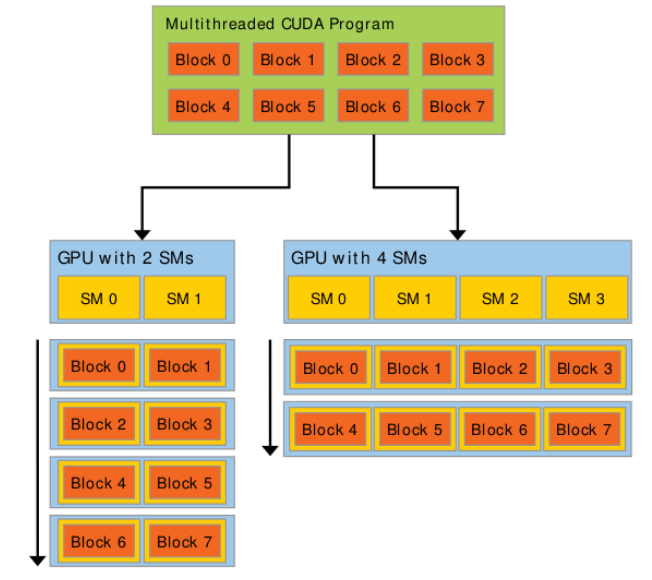
\includegraphics[width=0.8\textwidth]{images/cudaSMs.png}
		\caption{GPU scalability.}
		\label{fig:cudaSM}
	\end{figure}
	Indeed, \textit{each block of threads can be scheduled on any of the available SMs within a GPU, in any order, concurrently or sequentially}, so that a compiled CUDA program can execute on any number of multiprocessors as illustrated by Figure \ref{fig:cudaSM}, and only the runtime system needs to know the physical multiprocessor count.
	This programming model scales on the number of multiprocessors and memory partitions \cite{cudaguide}.  

\section{Profilers}	
	NVIDIA profiling tools were useful to optimize in performance our CUDA applications, we used three different versions: the \texttt{nvprof} profiling tool enables you to collect and view profiling data from the command-line. 
	
	%Note that Visual Profiler and nvprof will be deprecated in a future CUDA release. It is recommended to use next-generation tools NVIDIA Nsight Compute for GPU profiling and NVIDIA Nsight Systems for GPU and CPU sampling and tracing.
	
	%NVIDIA Nsight Compute is an interactive kernel profiler for CUDA applications. It provides detailed performance metrics and API debugging via a user interface and command line tool. In addition, its baseline feature allows users to compare results within the tool. Nsight Compute provides a customizable and data-driven user interface and metric collection and can be extended with analysis scripts for post-processing results.
	
	%NVIDIA Nsight Systems is a system-wide performance analysis tool designed to visualize an application’s algorithms, help you identify the largest opportunities to optimize, and tune to scale efficiently across any quantity or size of CPUs and GPUs; from large server to our smallest SoC.
	
	\subsection{nvprof}
%	CUDA Pro Tip: nvprof is Your Handy Universal GPU Profiler
%	By Mark Harris | October 23, 2013 Tags: CUDA, Development Tools and Libraries, GPU, Pro Tip, Profiling, Programming Languages and Compilers, Python, Tools
	\texttt{nvprof} was added to CUDA Toolkit with CUDA 5. It is a command-line profiler, so it's a GUI-less version of the graphical profiling features available in the NVIDIA Visual Profiler.\\
	The \texttt{nvprof} profiler enables the collection of a timeline of CUDA-related activities on both CPU and GPU, including kernel execution, memory transfers, memory set and CUDA API calls and events or metrics for CUDA kernels.\\
	After all data is collected, profiling results are displayed in the console \footnote{The textual output of the profiler is redirected to \texttt{stderr} by default.} or can be saved in a log file for later viewing \footnote{Or for later import into either \texttt{nvprof} or the \texttt{NVIDIA Visual Profiler)}.} \cite{profilersguide, nvprofarticle}.\\
	\texttt{nvprof} operates in different modes: \textit{Summary Mode}, \textit{GPU-Trace and API-Trace Modes}, \textit{Event/metric Summary Mode} and  \textit{Event/metric Trace Mode}.\\	
	For our purposes we used only \textit{Summary Mode}, this is the default operating mode, where we have a single result line for each kernel function and each type of CUDA memory copy performed by the application (for each operation type are shown number of calls and total, max, min and average time) \cite{profilersguide}.
	
	We used it, in some situations, as a quick check, for example we exploited it to see if the application wasn't running kernels on the GPU at all, or it was performing an unexpected number of memory copies, etc.
	To this aim it's enough to run the application with\\
	\texttt{nvprof ./myApp arg0 arg1 ...}\\
	Although when we launched our tests, we wanted to consult profiling results after running or whenever was necessary, it was useful especially when we had to compare them with time probes inside the code. So we used \texttt{--log-file} option to redirect the output to files for deferred examination. \\
	\texttt{nvprof} revealed peculiarly suitable for remote profiling. That's because of the fact command line is faster to check and save an application profiling.
	  
	\subsection{NVIDIA Visual Profiler}
	The NVIDIA Visual Profiler, introduced in 2008, is a performance profiling tool providing visual feedback for optimizing CUDA C/C++ applications.
	
	The Visual Profiler displays a timeline of an application's activity on both the CPU and GPU to make performance improvement, it analyzes the application to detect potential bottlenecks, using graphical views, that allow to check memory transfers, kernel launches, and other API functions on the same timeline \cite{profilersguide}.\\
	 
	We used the standalone version of the Visual Profiler, \texttt{nvvp}. 
	Furthermore we used NVIDIA Nsight Systems, the advanced version of Visual Profiler, this is a low overhead performance analysis tool that provides insights to optimize software, to investigate for bottlenecks. It also identifies issues, such as GPU starvation, unnecessary GPU synchronization, insufficient CPU parallelizing, unexpectedly expensive algorithms across the CPUs and GPUs of their target platform. 
	 
	In particular in this project \texttt{Nsight Systems} was used in developing phase, to check if code was properly written to hide as much as possible data transfers \footnote{We'll see in detail the Overlapping topic and how it was managed in \hyperref[chap:logic]{Chapter 3}.}, even though sometimes it may happens that profilers introduce some sampling synchronization, giving not fully reliable visual results.
	

\section{CUDA C/C++}
	Here we'll briefly introduce main concepts behind the CUDA programming model, by outlining how they are exposed in C.
	Especially we'll show important notions about features involved in this project and how/why these were included.
	\begin{wrapfigure}{l}{0.58\textwidth}
		\raggedleft
		
		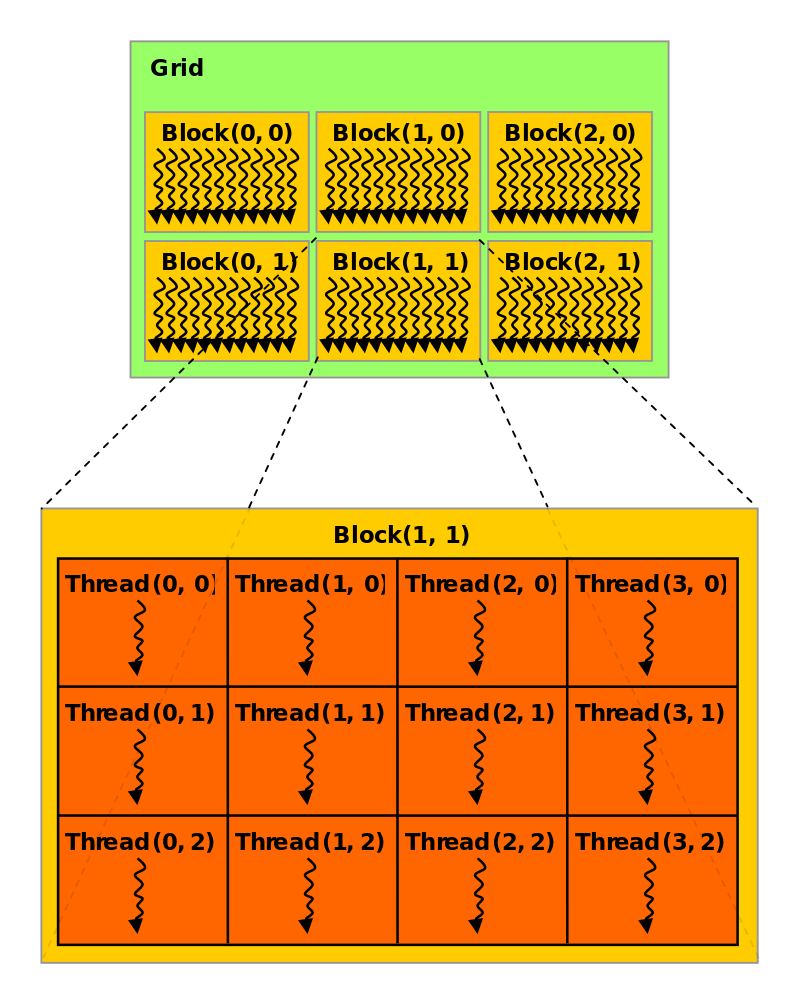
\includegraphics[width=0.58\textwidth]{images/gridblocks.png}
		\caption{Above: a Grid formed by Blocks.\\ Below: a Block formed by Threads.}
		\label{fig:gridblock}
	\end{wrapfigure}
	
	\subsection{Kernels} 
	\label{subs:ker}
	CUDA C allows to define particular C functions, called \textbf{\textit{kernels}}, when called, these are executed N times in parallel by N different CUDA threads, as	opposed to only once like regular C functions.
	
	A kernel is defined using the \texttt{\_\_global\_\_} declaration specifier. The number of CUDA threads that will execute the kernel for a given call is specified using this special execution configuration syntax: 
	\texttt{<<<...>>>}.\\
	Each thread executing the kernel is given a unique thread ID, accessible within the kernel through the built-in \texttt{threadIdx} variable \cite{cudaguide}.

	\subsection{Thread Hierarchy}  
	In practice \texttt{threadIdx} is a 3-component vector, so that threads can be identified using either one, or two, or three dimensional thread index.
	In turn these threads will form	either one, or two, or three dimensional block of threads, called a
	\textbf{\textit{thread block}}.
	This provides a way to invoke computation across the elements in domains such as a vectors, matrices, or volumes.
	%The index of a thread and its thread ID relate to each other in a straightforward way:
	%\begin{itemize}
	%	\item For a one-dimensional block, they are the same; 
		
	%	\item for a two-dimensional block of size \((D_{x} ,	D_{y}) \space \rightarrow \space\)  a thread of index \((x, y)\) has \(threadID = (x + y \cdot D_{x} );\)
		
	%	\item for a three-dimensional block of size \((D_{x} ,	D_{y} ,	D_{z}) \space \rightarrow \space\)  a thread of index \((x, y, z)\) has \(threadID = (x + y \cdot D_{x} + z \cdot D_{x} \cdot D_{y});\)
	%\end{itemize}
	There is a limit to the number of threads per block, since \textit{all threads of a block are expected to reside on the same processor core and must share the limited memory resources of that core}. On current GPUs, and on the two we worked on, a thread block may contain up to 1024 threads \footnote{see Table \ref{tab:gpuspecs} for limits in the machines we used).}.\\
	However, a kernel can be executed by multiple equally-shaped thread blocks, so that\\
	\(Total number of threads = \#threadsPerBlock \cdot \#blocks\)\\	 
	Blocks in turn are organized into either one, or two, or three dimensional \textit{\textbf{grid of thread blocks}} as illustrated by Figure \ref{fig:gridblock}.	
	So, the number of blocks in a grid is usually dictated by the size of the data being processed or the number of processors in the system.
	The number of \textit{threads per block} and the number of \textit{blocks per grid} specified in the 	\texttt{<<<...>>>} syntax can be of type \texttt{int} or \texttt{dim3}.\\
	The dimension of the thread block, block index and thread index are accessible within the kernel through the respective built-in variables: \texttt{blockDim}, \texttt{blockIdx}, \texttt{threadIdx}. \cite{cudaguide}.

	\subsection{CUDA Streams}
	\label{subs:streams} 
	\textbf{Overlap of Data Transfer and Kernel Execution}\\
	Some devices can perform an asynchronous memory copy to or from the GPU	concurrently with kernel execution. 
	It's possible to query this capability by checking the \texttt{asyncEngineCount} device property \footnote{ See \textit{Device Enumeration} in Table \ref{tab:gpuspecs}, For both of our machines, from the \textit{deviceQuery}, we get 2 copy engines.}, which is greater than zero for devices that support it. If host memory is involved in the copy, it must be
	\textit{\textbf{page-locked}}.\\\\
	%In particular some devices, of compute capability 2.x and higher, can overlap copies to and from the device. Applications may query this capability by checking the \texttt{asyncEngineCount} device property (see Device Enumeration), which is equal to 2 for devices that support	it \footnote{This is the case for both of our machines. \\ See the last line of \texttt{deviceQuery} in Table \ref{tab:gpuspecs}}. 
	\Large \textbf{Streams}\normalsize\\
	Applications manage the concurrent operations described above through \textbf{streams}. A stream is a sequence of commands (possibly issued by different host threads) that execute in order. On the other hand, a stream may execute their commands out of order or concurrently with respect to another; this behavior is not guaranteed and	should not be relied upon for correctness (e.g. inter-kernel communication is undefined) \cite{cudaguide}.\\
	A brief code example:
	\begin{lstlisting}[caption={CUDA Strams creation}]
	cudaStream_t stream[2];
	for (int i = 0; i < 2; ++i)
		cudaStreamCreate(&stream[i]);
	float* hostPtr;
	cudaMallocHost(&hostPtr, 2 * size);
	\end{lstlisting}	

	Each of these streams is defined, by the following code sample, as a sequence of one memory copy \(host \rightarrow device\), one kernel launch, and one memory copy \(host \leftarrow device\):
	\begin{lstlisting}[caption={CUDA Strams and Async example}]
	for (int i = 0; i < 2; ++i) {
		cudaMemcpyAsync(inputDevPtr + i * size, hostPtr + i * size, size, cudaMemcpyHostToDevice, stream[i]);
		MyKernel <<<100, 512, 0, stream[i]>>> (outputDevPtr + i * size, inputDevPtr + i * size, size);
		cudaMemcpyAsync(hostPtr + i * size, outputDevPtr + i * size, size, cudaMemcpyDeviceToHost, stream[i]);
	}
	\end{lstlisting}
	
	Each stream copies its portion of input array \texttt{hostPtr} to array \texttt{inputDevPtr} in device memory, processes \texttt{inputDevPtr} on the device by calling \texttt{MyKernel()}, and copies
	the result \texttt{outputDevPtr} back to the same portion of \texttt{hostPtr}. Note that \texttt{hostPtr} must point to page-locked host memory for any overlap to
	occur.\\
	Streams are released by calling \texttt{cudaStreamDestroy()}.
	\begin{lstlisting}[caption={CUDA Strams destroy}]
	for (int i = 0; i < 2; ++i)
		cudaStreamDestroy(stream[i]);
	\end{lstlisting}
	
%	In case the device is still doing work in the stream when cudaStreamDestroy() is 	called, the function will return immediately and the resources associated with the stream 	will be released automatically once the device has completed all work in the stream.


%	3.2.5.5.2. Default Stream
%	Kernel launches and host <-> device memory copies that do not specify any stream
%	parameter, or equivalently that set the stream parameter to zero, are issued to the default
%	stream. They are therefore executed in order.
%	For code that is compiled using the --default-stream per-thread compilation flag
%	(or that defines the CUDA\_API\_PER\_THREAD\_DEFAULT\_STREAM macro before including
%	CUDA headers ( cuda.h and cuda\_runtime.h )), the default stream is a regular stream
%	and each host thread has its own default stream.
%	For code that is compiled using the --default-stream legacy compilation flag, the
%	default stream is a special stream called the NULL stream and each device has a single
%	NULL stream used for all host threads. The NULL stream is special as it causes implicit
%	synchronization as described in Implicit Synchronization.
%	For code that is compiled without specifying a --default-stream compilation flag, --
%	default-stream legacy is assumed as the default.
	
%	QUESTO LO METTEREI NEL CAPITOLO IMPLEMENTATION
%	3.2.5.5.3. Explicit Synchronization
%	There are various ways to explicitly synchronize streams with each other.
%	cudaDeviceSynchronize() waits until all preceding commands in all streams of all
%	host threads have completed.
%	cudaStreamSynchronize() takes a stream as a parameter and waits until all preceding
%	commands in the given stream have completed. It can be used to synchronize the host
%	with a specific stream, allowing other streams to continue executing on the device.
%	www.nvidia.com
%	CUDA C Programming Guide
%	PG-02829-001\_v10.0 | 33Programming Interface
%	cudaStreamWaitEvent() takes a stream and an event as parameters (see Events for
%	a description of events)and makes all the commands added to the given stream after
%	the call to cudaStreamWaitEvent() delay their execution until the given event has
%	completed. The stream can be 0, in which case all the commands added to any stream
%	after the call to cudaStreamWaitEvent() wait on the event.
%	cudaStreamQuery() provides applications with a way to know if all preceding
%	commands in a stream have completed.
%	To avoid unnecessary slowdowns, all these synchronization functions are usually best
%	used for timing purposes or to isolate a launch or memory copy that is failing.
%	3.2.5.5.4. Implicit Synchronization
%	Two commands from different streams cannot run concurrently if any one of the
%	following operations is issued in-between them by the host thread:
%
%	-a page-locked host memory allocation,
%	-a device memory allocation,
%	-a device memory set,
%	-a memory copy between two addresses to the same device memory,
%	-any CUDA command to the NULL stream,
%	-a switch between the L1/shared memory configurations described in Compute
%	Capability 3.x and Compute Capability 7.x.
%	For devices that support concurrent kernel execution and are of compute capability 3.0
%	or lower, any operation that requires a dependency check to see if a streamed kernel
%	launch is complete:
%
%	-Can start executing only when all thread blocks of all prior kernel launches from any
%	stream in the CUDA context have started executing;
%	-Blocks all later kernel launches from any stream in the CUDA context until the kernel launch being checked is complete.
%	Operations that require a dependency check include any other commands within the
%	same stream as the launch being checked and any call to cudaStreamQuery() on that
%	stream. Therefore, applications should follow these guidelines to improve their potential
%	for concurrent kernel execution:
%	-All independent operations should be issued before dependent operations,
%	-Synchronization of any kind should be delayed as long as possible.
%	3.2.5.5.5. Overlapping Behavior
%	The amount of execution overlap between two streams depends on the order in which
%	the commands are issued to each stream and whether or not the device supports
%	overlap of data transfer and kernel execution (see Overlap of Data Transfer and Kernel
%	Execution), concurrent kernel execution (see Concurrent Kernel Execution), and/or
%	concurrent data transfers (see Concurrent Data Transfers).
%	For example, on devices that do not support concurrent data transfers, the two streams
%	of the code sample of Creation and Destruction do not overlap at all because the
%	www.nvidia.com
%	CUDA C Programming Guide
%	PG-02829-001\_v10.0 | 34Programming Interface
%	memory copy from host to device is issued to stream[1] after the memory copy from
%	device to host is issued to stream[0], so it can only start once the memory copy from
%	device to host issued to stream[0] has completed. If the code is rewritten the following
%	way (and assuming the device supports overlap of data transfer and kernel execution)
%	for (int i = 0; i < 2; ++i)
%	cudaMemcpyAsync(inputDevPtr + i * size, hostPtr + i * size,
%	size, cudaMemcpyHostToDevice, stream[i]);
%	for (int i = 0; i < 2; ++i)
%	MyKernel<<<100, 512, 0, stream[i]>>>
%	(outputDevPtr + i * size, inputDevPtr + i * size, size);
%	for (int i = 0; i < 2; ++i)
%	cudaMemcpyAsync(hostPtr + i * size, outputDevPtr + i * size,
%	size, cudaMemcpyDeviceToHost, stream[i]);
%	then the memory copy from host to device issued to stream[1] overlaps with the kernel
%	launch issued to stream[0].
%	On devices that do support concurrent data transfers, the two streams of the code
%	sample of Creation and Destruction do overlap: The memory copy from host to device
%	issued to stream[1] overlaps with the memory copy from device to host issued to
%	stream[0] and even with the kernel launch issued to stream[0] (assuming the device
%	supports overlap of data transfer and kernel execution). However, for devices of
%	compute capability 3.0 or lower, the kernel executions cannot possibly overlap because
%	the second kernel launch is issued to stream[1] after the memory copy from device
%	to host is issued to stream[0], so it is blocked until the first kernel launch issued to
%	stream[0] is complete as per Implicit Synchronization. If the code is rewritten as
%	above, the kernel executions overlap (assuming the device supports concurrent kernel
%	execution) since the second kernel launch is issued to stream[1] before the memory copy
%	from device to host is issued to stream[0]. In that case however, the memory copy from
%	device to host issued to stream[0] only overlaps with the last thread blocks of the kernel
%	launch issued to stream[1] as per Implicit Synchronization, which can represent only a
%	small portion of the total execution time of the kernel.
		 
	\subsection{nvcc compiler}
	To compile the CUDA C++ code was necessary to use a special compiler, included in CUDA Toolkit, that is \texttt{nvcc}.\\
	The CUDA compiler driver hides the details of CUDA compilation from developers. It accepts a range of conventional compiler options, for example for the project we could define macros or include library paths \footnote{NVCC documentation: https://docs.nvidia.com/cuda/cuda-compiler-driver-nvcc/index.html\#introduction}.\\ 
	All non-CUDA compilation steps are forwarded to a C++ host compiler that is supported by \texttt{nvcc}. 
	Source files compiled with \texttt{nvcc} can include a mix of host code and device code. \texttt{nvcc}'s basic
	workflow consists in separating device from host code and then:
	\begin{itemize}
		\item compiling the device code into an assembly form (PTX code) and/or binary form (cubin object), \item and modifying the host code by replacing the \texttt{<<<...>>>} syntax introduced in	Kernels \footnote{See  \hyperref[subs:ker]{subsection 2.3.1}} by the necessary CUDA C runtime function calls, to load and launch each compiled kernel from the PTX code and/or cubin object.
	\end{itemize}
	The modified host code is output either as C code that is left to be compiled using another tool, or as object code directly by letting \texttt{nvcc} invoke the host compiler during	the last compilation stage.
	Applications can then either link to the compiled host code (most common case), or ignore the modified host code (if any) and use the CUDA driver API to load and execute the PTX code or cubin object.\\
	This compiler can be used almost the same way as a classic \texttt{gcc}, for example:
	
	\texttt{nvcc -std=c++14 -g -G -o executable source.cu}\\	
	Here we present compiler versions installed in our two machines:	
	\begin{itemize}
		\item \textbf{Tesla P100}\\
		nvcc: NVIDIA (R) Cuda compiler driver, 
		%Copyright (c) 2005-2019 NVIDIA Corporation
		%Built on Wed_Apr_24_19:10:27_PDT_2019
		%Cuda compilation tools,
	 release 10.1, V10.1.168			
		 
		\item \textbf{Tesla M40}\\
	 nvcc: NVIDIA (R) Cuda compiler driver, 
	 %Copyright (c) 2005-2019 NVIDIA Corporation
	 %Built on Fri_Feb__8_19:08:17_PST_2019
	 %Cuda compilation tools, 
	 release 10.1, V10.1.105
	\end{itemize}
		 
	\subsection{\texttt{cuda-gdb} debugger}
	\texttt{CUDA-GDB} is the NVIDIA tool for debugging CUDA applications (available on Linux). It is an extension to the x86-64 port of GDB, the GNU Project debugger.\\
	Cuda-gdb main features are:
	\begin{itemize}
		\item it gives environment that allows simultaneous debugging of both GPU and CPU code within the same application;
		
		\item as programming in CUDA C is an extension to C programming, debugging with CUDA-GDB is an extension to debugging with GDB, so the existing GDB debugging features are present for debugging the host code (additional features have been provided to support  CUDA device code);	
		
		\item it allows to set breakpoints, to single-step CUDA applications, and also to inspect and modify the memory and variables of any given thread running on the hardware;
		
		\item it supports debugging all CUDA applications, whether they use the CUDA driver API, the CUDA runtime API, or both.
		
		\item it supports debugging kernels that have been compiled for specific CUDA architectures, but also supports debugging kernels compiled at runtime, referred to as just-in-time (JIT) compilation.
	\end{itemize}	
	\texttt{CUDA-GDB} was used to debug all compiled source files, both \texttt{.cu} and \texttt{.cpp} .
	Mainly it was really helpful in this project to step device code, inspect runtime errors thrown by CUDA API calls and check exactly what code was doing inside our kernels.
	
\section{Visual Studio Code}
	Visual Studio Code is an open-source code editor by Microsoft for Linux Operative Systems too. It includes support for debugging, embedded Git control and GitHub, syntax highlighting, intelligent code completion, snippets, and code refactoring \footnote{Other infos: https://en.wikipedia.org/wiki/Visual\_Studio\_Code \\
		Documentation: https://docs.microsoft.com/it-it/dotnet/core/tutorials/with-visual-studio-code \\ 
		Website: https://code.visualstudio.com/}.\\
	Since it's customizable we could add C++ and CUDA editor extensions, furthermore an SFTP extension allowed us to quickly upload/download files from remote machines. 	
	
\section{Tests, Result gathering, Plots}
Some other peripheral tools were involved in this project.
In particular we needed:
\begin{itemize}
	\item a way to serially run executions of our applications,possibly varying input dataset on interest values;
	\item put all results on text files;
	\item implement a script to compute averages, speedups and other interest metrics, from results on text files;
	\item a generator of graphs on important values from the obtained calculations.
\end{itemize}

\subsection{Bash scripts}
\label{subs:bash}
Bash (Bourne-Again SHell) is the shell, or command language interpreter, for the GNU operating system; the latter provides other shells, but Bash is the default  shell\footnote{https://www.gnu.org/software/bash/manual/}. 

\textbf{\texttt{Bash scripts}} were needed to implement tests, that run more executions of a certain CUDA application, also varying input dataset.
We programmed bash scripts (\texttt{.sh}) tests to contain several command as compile a certain CUDA application, run many times the related executable, profile it with \texttt{nvprof} and so on.

\subsection{Python scripts}
As Python \footnote{The Python version used to compile, on local host, our scripts is: Python 2.7.6.\\ See documentation: https://docs.python.org/2/} has dynamic typing, together with its interpreted nature, it's an ideal language for scripting and rapid application development.

In the case of this work was most useful to quickly implement a result filter: given text files with time measures, we computed averages and some speedups. \\
Furthermore we implemented a script to generate some plots on averages and speedups, exploiting the library \texttt{matplotlib} \footnote{https://matplotlib.org/}




